\section{Applications}

\begin{figure}[!t]
\centering
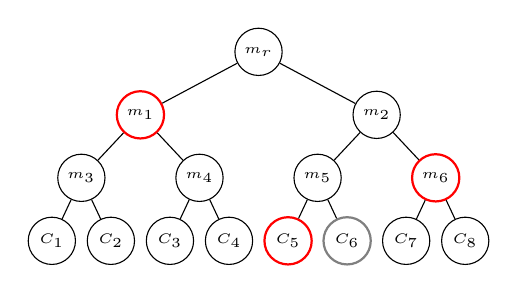
\begin{tikzpicture}[
    level 1/.style={sibling distance=30mm, level distance=8mm},
    level 2/.style={sibling distance=15mm, level distance=8mm},
    level 3/.style={sibling distance=7.5mm, level distance=8mm},
    every node/.style={draw, circle, minimum size=6mm, inner sep=0pt, font=\tiny}
]
    % Root node
    \node {$m_r$}
        % Level 1
        child {node[draw=red, line width=0.8pt] {$m_1$}
            % Level 2
            child {node {$m_3$}
                % Level 3
                child {node {$C_1$}}
                child {node {$C_2$}}
            }
            child {node {$m_4$}
                % Level 3
                child {node {$C_3$}}
                child {node {$C_4$}}
            }
        }
        child {node {$m_2$}
            % Level 2
            child {node {$m_5$}
                % Level 3
                child {node[draw=red, line width=0.8pt] {$C_5$}}
                child {node[draw=gray, line width=0.8pt] {$C_6$}}
            }
            child {node[draw=red, line width=0.8pt] {$m_6$}
                % Level 3
                child {node {$C_7$}}
                child {node {$C_8$}}
            }
        };
\end{tikzpicture}
\caption{Merkle tree with authentication path (in red) for deposit commitment $C_6$ (in gray) used by applications like Tornado cash. Here, $C_6$ is recursively hashed with its children all the way to the root. If the computed root matches $m_r$ at deposit time, then the user is allowed to withdraw the amount of funds specified in $C_6$.}
\label{fig:merkle-tree}
\end{figure}

\subsection{Application/Infrastructure-Level Privacy Preservation}
\noindent Traditional blockchain network innerworkings expose transaction details, making privacy preservation nontrivial at the application/infrastructure layers. Applications like Tornado Cash \cite{tornadocash} partially solve this problem at the application layer, using groth16 proofs to enable privacy-preserving deposits and withdrawals to different wallets without revealing the link between the two. Withdrawing funds involves proving membership of one's deposit record in a Merkle tree, as shown in figure \ref{fig:merkle-tree}; combined with tight EVM smart contract gas limits, the homogeneous nature of this computation makes groth16 a suitable choice. Blockchains like Zerocash \cite{zcash} (privacy-preserving version of Bitcoin \cite{bitcoin}) somewhwat generalize tornado cash's abilities using the unspent transaction output (UTXO) model, where spending funds requires proving knowledge of an ``unspent funds'' record in a Merkle tree. Early versions of Zerocash used groth16 for this, but the NU5 upgrade of 2022 switched to the universal halo2 proof system \cite{halo2}, which enables a combination of a PlonK-style arithmetization and Bulletproofs-style commitment scheme \cite{bulletproofs} requiring no trusted setup at the expense of verifier performance. Beyond such homogeneous computation, non-universal (zk)SNARKs could be used for application-specific privacy-preserving blockchains as well (ex. a blockchain for private trading/lending). 

\subsection{zkVMs and ``Layer-2'' Scaling Solutions for Ethereum Network}
\noindent Layer-2 (L2) blockchains \cite{l2survey} have emerged as a dominant scaling solution to layer-1 (L1) chains like Ethereum \cite{ethereum}. These alternate blockchains are essentially Ethereum forks with their own application layer and transaction processing; however, they settle batches of transactions directly on Ethereum network. These alternate outlets afford users a similar experience while easing computational load on the Ethereum chain. ``Zero-knowledge'' virtual machines (zkVMs) \cite{scrollzkevm, polygonzkevm, sp1, risc0, openvm} are a crucial component of this architecture, as they produce succinct proofs of L2 block validity which are later settled by verifier contracts on the L1 chain. zkVMs using PlonK variants \cite{scrollzkevm} have already played a huge role in the functionality of zkVMs powering widely used L2 chains \cite{scrollarch}. Further advancements in lookup arguments based on either PlonK or other methods will have huge impacts on transaction processing speed, layer 2 network performance, and ultimately the scalability of Ethereum network itself.  

% \noindent A crucial point of consideration here is that not all computations performed in VVMs are ``SNARK-friendly''; a prime example of this is hash functions like SHA256 which use non-linear or non-algebraic operations like bit mixing. This can cause the circuits constraining this computation to be overly complex and inefficient. To meet this end, lookup-based methods are of great interest here since they can avoid constraining ``SNARK-unfriendly'' operations directly without losing soundness. An example of this is lies in the proof for validity of transaction that called a contract function using \texttt{sha256()}. Instead of constraining the exact sha-256 computation, the prover and verifier would agree on a publicly known table of acceptable inputs and outputs for SHA-256, which the prover commits to as part of the proof. The verifier does not need to know the whole table - they just need to know a commitment to the one considered correct. This can then be compared with what the prover committed to.\\
